En esta sección abordaremos el problema del viajante de comercio. Dado que
se trata de un algoritmo de clase NP, es prácticamente inviable encontrar 
un algoritmo que encuentre la solución óptima en un tiempo razonable.

Por tanto, para abordar este problema se emplearán 3 heurísticas diferentes que,
si bien no siempre encuentran la solución óptima, determinan soluciones 
aceptables en tiempos razonables. Para cada una de
estas heurísticas se comparará su rendimiento en un conjunto de prueba,
midiendo los tiempos de ejecución. 

\subsection{Descripción de las heurísticas}

En esta sección se realizará una descripción de cada heurística que hemos 
empleado, incluyendo tanto algoritmos, implementación como casos de ejemplo.
Dos heurísticas han sido proporcionados por los profesores: el \textit{vecino
más cercano} e \textit{inserción}, mientras que la tercera es de
elaboración propia.

\subsubsection{Vecino más cercano}

\begin{figure}[H] 
  \centering
  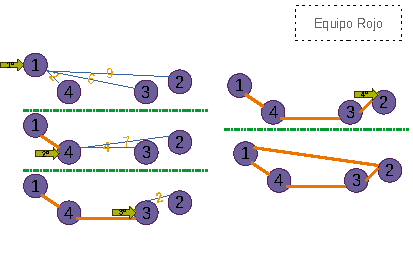
\includegraphics[scale=1.5]{img/DibVecCercano.pdf}
  \caption{Ilustración del funcionamiento de la heurística del vecino más cercano.}
  \label{fig:vec}
\end{figure}

La filosofía que gobierna esta heurística es bastante sencilla. La idea 
radica en ir insertando ciudades en el conjunto de solución $S$, de manera
que para decidir la ciudad $c_{i+1}$ que se insertará se escoge aquella que
dista la menor distancia de la ciudad $c_i$ (para $c_0$ se escoge
un nodo al azar). Esta idea queda resumida en el Algoritmo~\ref{alg:vec_cercano}. 

\begin{algorithm}
    \caption{Algoritmo del vecino más cercano, para el TSP}\label{alg:vec_cercano}
    $vector<int> candidates,result$\;
    index\;
    $i \gets 0$\;
    $size \gets v[0].size$\;

    $candidates.push\_back(i)$\;

    \While{$candidates.size < size$}{
      $index \gets nearest\_point(v[i],candidates)$\;
      $candidates.push\_back(index)$\;
      $i \gets index$\;
    }
\end{algorithm}

Una implementación del algoritmo propuesto está expuesto en el Código~\ref{cod:vec}. 

\lstinputlisting[label={cod:vec}, firstline=70, lastline=118, language=C++,
caption=Implementación del algoritmo del vecino más cercano en TSP.]{../src/tsp.cpp}

\subsubsubsection{Análisis de eficiencia}

La variable respecto al cual realizamos el análisis de eficiencia teórico es el número
de ciudades $n$. Consideramos simultáneamente tanto la función maestra como la función
auxiliar de este algoritmo para el análisis. 

Las operaciones tanto antes como después del bucle \texttt{while} son operaciones constantes
donde no influye el número total de ciudades $n$ y pueden ser acotadas por una
constante. Dentro del bucle, tenemos que
el primer bucle  \texttt{while} realiza $kn$ con iteraciones de otro bucle \texttt{for}, con 
$k \in \mathbb Z$ constante. A su vez, dentro de este bucle for (dentro de la función auxiliar) 
también se realizan n repeticiones,
por lo que se realiza un total de $k'n$ operaciones elementales dentro de ella, 
con $k' \in \mathbb Z$ constante. Por tanto, tenemos que su orden de 
eficiencia es $\boxed{\mathcal O(n^2)}$. 

\subsubsection{Inserción económica}

\begin{figure}[H] 
  \centering
  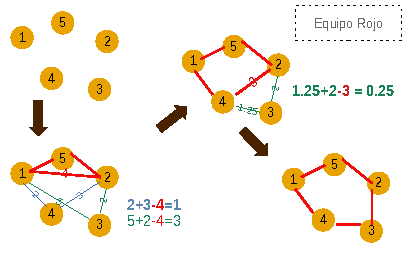
\includegraphics[scale=1.5]{img/DibInsercion.pdf}
  \caption{Ilustración del funcionamiento de la heurística de inserción.}
  \label{fig:inser}
\end{figure}

En este caso para obtener la solución final se fijan $c_1,c_2,c_3$ ciudades
(siguiendo las indicaciones de la práctica, se han
escogido las ciudades situadas más al norte, este y oeste). 
Posteriormente,
para decidir la ciudad $c_{i+1}$ que se insertará en el conjunto de solución,
se elige aquella que, al insertarse en un determinado arco del ciclo 
$0 \leq j \leq i$, minimice la variación en el ciclo formado por las ciudades
$c_1,c_2,\cdots,c_{i}$. Dicha ciudad se añade intercalado entre las ciudades
$c_{j},c_{j+1}$. El algoritmo asociado a esta heurística se encuentra en 
Algoritmo~\ref{alg:insercion}. 

\begin{algorithm}[H]
  \caption{Algoritmo auxiliar para la inserción. InsercionEconomica}\label{alg:insercion-aux-1}
  \begin{minipage}{0.92\textwidth}
    \textbf{Parámetro}: ady (matriz de adyacencia)

    \textbf{Parámetro}: ciclo (solución parcial)

    \textbf{Parámetro}: pos
  \end{minipage}

  $(c_{ini}, c_{fin}) = (-1,-1)$\;
  $var = \infty$\;
  ind = -1\;

  \For{i desde 0 hasta ciclo.size-1}{
    $(c_a, c_b)$ = ciclo[i]\;
    nueva\_variacion = $ady[c_a][c_i] + ady[c_i][c_b] - ady[c_a][c_b]$\;

    \If{nueva\_variacion $<$ variacion}{
      $(c_{ini}, c_{fin}) = (c_a, c_b)$\;
      ind = i\;
    }
  }
  
  \Return{$(ind, pos, var)$}
\end{algorithm}

\begin{algorithm}[H]
  \caption{Algoritmo auxiliar para la inserción. CiudadEconomica (se usa el Algoritmo~\ref{alg:insercion-aux-1})}\label{alg:insercion-aux-2}
  \begin{minipage}{0.92\textwidth}
    \textbf{Parámetro}: ady (matriz de adyacencia)

    \textbf{Parámetro}: ciclo (solución parcial)

    \textbf{Parámetro}: banderas
  \end{minipage}

  ind = 0\;

  \While{banderas[ind] e ind valido}{
    ind++\;
  }

  $(ind_a, pos_a, var_a)$ = InsercionEconomica(ady,ciclo,ind)\;

  \For{i desde ind+1 hasta ady.tamaño}{
    \If{banderas[i] no activado}{
      $(ind_n, pos_n, var_n)$ = InsercionEconomica(ady, ciclo, i)\;
      % $(c_{n}, c_{n+1}, var_n)$ = InsercionEconomica(ady, ciclo, i)\;

      \If{$var_n < var_a$ }{
        $(ind_a, pos_a, var_a)$ = $(ind_n, pos_n, var_n$\;
      }
    }
  }

  \Return{$(c_{ind_a},pos_a)$}
  
\end{algorithm}

El Algoritmo~\ref{alg:insercion-aux-1} y el Algoritmo~\ref{alg:insercion-aux-2}
se emplean como funciones auxiliales sobre los que se basa el algoritmo maestro. 

Se presenta el algoritmo máster.

\begin{algorithm}[H]
    \caption{Algoritmo basado en inserción. CicloInsercionEconomica (se usan los algoritmos 
    auxiliares Algoritmo~\ref{alg:insercion-aux-1} y Algoritmo~\ref{alg:insercion-aux-2})}\label{alg:insercion}
    \begin{minipage}{0.92\textwidth}
      \textbf{Parámetro}: puntos (vector de posiciones)
      
      \textbf{Parámetro}: ady (matriz de adyacencia)
    \end{minipage}
    % $Ady = MatrizAdyacencia(C)$\;
    % $N = C.\text{tamaño}$\;
    % $S = []$\;
    % $S$.añadir($c_\alpha$), con $\alpha \in \{j \in \mathbb N : c_j.x \geq c.x, \forall c \in C\}$ \Comment*[r]{Ciudad más al este}
    % $S$.añadir($c_\beta$), con $\beta \in \{j \in \mathbb N : c_j.x \leq c.x, \forall c \in C\}$ \Comment*[r]{Ciudad más al oeste}
    % $S$.añadir($c_\gamma$), con $\gamma \in \{j \in \mathbb N : c_j.y \geq c.y, \forall c \in C\}$ \Comment*[r]{Ciudad más al norte}
    % \While{$S.\text{tamaño} \leq N$}{
    %   $(i,pos) = CiudadEconomica(C, S, Ady)$\;
    %   $S$.insertar(pos, $c_i$)\;
    %   $C$.quitar($c_i$)\;
    % }

    ciclo = []\;

    N = puntos.tamaño;
    Banderas = []\;

    \For(){i desde 0 hasta N-1}{
      Banderas.insertar(false)
    }

    \Comment*{Añadimos las tres primeras ciudades}

    ind\_este = IndCiudadEste(puntos);
    banderas[ind\_este] = true\;

    ind\_oeste = IndCiudadOeste(puntos);
    banderas[ind\_oeste] = true\;

    ind\_este = IndCiudadNorte(puntos);
    banderas[ind\_norte] = true\;


    ciclo.insertar((ind\_este, ind\_oeste));
    ciclo.insertar((ind\_oeste, ind\_norte))\;
    ciclo.insertar((ind\_norte, ind\_este))\;

    % $S$.añadir(puntos[ind_este])\;
    % $S$.añadir(puntos[ind_oeste])\;
    % $S$.añadir(puntos[ind_norte])\;

    \Comment*{Añadimos el resto de ciudades}
    \For(){i desde 3 hasta N-1}{
      $(c_i,pos)$ = CiudadEconomica(ady, ciclo, banderas)\;
      $(c_j, c_{j+1})$ = s[pos]\;
      banderas[$c_i$] = true\;
      ciclo.insertar(pos, $(c_i,c_{j+1})$)\;
      ciclo.insetar(pos, $(c_j,c_i)$)\;
    }
    \Return{ciclo}
\end{algorithm}

El código asociado al algoritmo Algoritmo~\ref{alg:insercion} viene especificado
a continuación, en el Código~\ref{cod:tsp1}. 

\lstinputlisting[label={cod:tsp1}, firstline=119, lastline=300, language=C++,
caption=Implementación del algoritmo de inserción en TSP.]{../src/tsp.cpp}

\subsubsubsection{Análisis de eficiencia}

Los algoritmos para encontrar las ciudades situadas más al norte, este y oeste
recorren todas las ciudades, realizando operaciones constante, por lo que este
primer bloque tiene eficiencia $O(n)$. El siguiente bucle for realiza un número de operaciones
independiente del número total de ciudades a considerar. El siguiente for ya sí
influye en el análisis del rendimiento. A medida que va avanzando el índice,
el número de operaciones que se realizan en la función auxiliar aumenta, de la
forma que se realizan las siguientes operaciones, con $k,k' \in \mathbb Z$ constantes.
Cada paréntesis representa las operaciones que se realizan en una iteración del ciclo for.

\begin{equation*}
  T(n) = (k + k'·n·3) + (2 k + k'·n·4) + \cdots + ((n-3)k + k'·n·(n) = k (1 + 2 +3 +\cdots + (n-3)) + nk'(3+4+\cdots+n)
\end{equation*}

Desarrollamos:

\begin{equation*}
  T(n) = k \frac{(n-3)(n-2)}{2} + nk' \frac{(n-3)(n+3)}{2} \Rightarrow \boxed{T(n) \in \mathcal O(n^3)}
\end{equation*}

\subsubsection{Heurística basada en el algoritmo de Kruskal} 

\begin{figure}[H] 
  \centering
  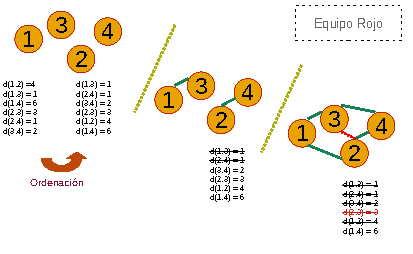
\includegraphics[scale=1.5]{img/DibPropio.pdf}
  \caption{Ilustración del funcionamiento de la heurística propia, basada en el algoritmo de Kruskal.}
  \label{fig:vec}
\end{figure}

La siguiente heurística de elaboración propia se basa en la idea utilizada en el \textbf{algoritmo de Kruskal} para la determinación del AGM. 

Dado el conjunto de $n$ ciudades conectadas entre sí, se crea un grafo $G$ que represente la red de ciudades, y un grafo $S$ que en el momento de su construcción contenga únicamente las ciudades o nodos de $G$, pero sin ninguna conexión entre nodos.

A continuación, ordenamos los arcos de $G$ en orden creciente según la ponderación del arco (sin incluir lazos, es decir, ciclos entre un nodo y el mismo). Esta \textbf{lista de arcos}, $L$, constituye nuestro \textbf{conjunto de candidatos}, es decir en cada etapa del algoritmo, \textbf{la función de selección escoge el arco de menor ponderación} (primer elemento de la lista), y seguidamente comprobamos si el arco escogido cumple las condiciones de factibilidad, si las cumple será insertado en $S$, y en caso contrario ese arco será descartado de la solución. 

En cuanto a la factibilidad de un candidato, tenemos \textbf{dos condiciones de factibilidad}. La primera consiste en comprobar que los nodos entre los que vamos a insertar el arco cumplen la siguiente condición: el nodo origen debe de tener como máximo un nodo incidente, y no puede tener un arco adyacente, y el nodo destino debe de tener como máximo un arco adyacente y no debe tener un arco incidente. Con esta condición nos garantizamos parte de la construcción de un circuito en el grafo $S$, de forma que \textbf{cada nodo del grafo solución tenga una única entrada y una única salida}. La segunda condición consiste en comprobar que al añadir el arco candidato al grafo solución $S$ \textbf{no se formen ciclos}, aunque esta condición no se comprueba en la última iteración del algoritmo, ya que debe formarse un circuito en la última etapa.

El algoritmo terminará cuando se hayan insertado tantas aristas como nodos tiene $S$, formando un circuito Hamiltoniano. La elección del arco de menor coste entre los que hay disponibles responde a la idea de intentar minimizar la \textbf{función objetivo}, que mide el coste total del circuito.

\begin{algorithm}
	\caption{Algoritmo basado en Kruskal}\label{alg:bas_kruscal}
	\begin{minipage}{0.92\textwidth}
		\textbf{Parámetro}: L (lista de arcos ordenada)
		
		\textbf{Parámetro}: nNodos (número de nodos/ciudades)
		
		\textbf{Parámetro}: grafoSol (grafo con la solución, parámetro de entrada/salida)
	\end{minipage}

  S = $\{\}$\;
  nArcos = 0\;
  
  \While{nArcos < nNodos y L.novacio}{
    arcoCandidato = L.frente()\;
    L.eliminaFrente()\;

    \eIf{nArcos == nNodos-1}{
      \If{nodosCorrectos(arcoCandidato.origen,arcoCandidato.destino)}{
        S = S $\cup$ $\{$arcoCandidato$\}$\;
        nArcos++\;
      }
    }{
      \eIf{nodosCorrectos(arcoCandidato.origen,arcoCandidato.destino)}{
        S = S $\cup$ $\{$arcoCandidato$\}$\;
        \If{sinCiclos(solucion)}{
          nArcos++\;
        }
      }{
        nOrigen = buscarNodoConIndice(arcoCandidato.origen)\;
        nDestino = buscarNodoConIndice(arcoCandidato.destino)\;
        borrarAdyacencia(nOrigen)\;
        borrarIncidencia(nDestino)\;
      }
    }
  }

  \Return{S}
\end{algorithm}

\lstinputlisting[label={cod:cod-e2c}, firstline=7, lastline=145, language=C++,
caption=Implementación del algoritmo de TSP basado en Kruskal.]{../src/ejercicio-2-c.cpp}

\subsubsubsection{Análisis de eficiencia}

Empecemos con el análisis teórico, analizando la eficiencia asintótica $big(O)$. Llamaremos $n$ al número 
de nodos del grafo que representa la red. La función que se encargar de obtener el circuito hamiltoniano 
solución \texttt{resuelvePVC}, tiene un bucle \texttt{while} que realizará $n$ iteraciones. Dentro del mismo, 
la función \texttt{buscarNodoConIndice} tiene eficiencia $O(n)$, y también en el interior del bucle, la 
función \texttt{sinCiclos} tiene una eficiencia $O(n^2)$, luego \textbf{la eficiencia de \texttt{resuelvePVC} es $O(n^3)$}.

\subsubsubsection{Estudio de los tiempos de cada algoritmo}

Estudiando los tiempos de cada algoritmo nos damos cuenta de que el algoritmo proporcionado por nosotros es el más ineficiente
con bastante diferencia respecto a los otros dos, siendo el del vecino el algoritmo que menos tarda en ejecutarse.

\begin{table}[H]
  \centering
  \begin{tabular}{|c|c|c|c|}
    \hline
    & bayg & eil & ulysses \\
    \hline
    vecino más cercano & 76 & 248 & 39 \\
    \hline
    inserción & 402 & 2240 & 120 \\
    \hline
    $\alpha$-Kruskal & 8859 & 16048 & 2559 \\
    \hline
  \end{tabular}
  \caption{Tabla donde se indica el tiempo empleado en microsegundos en los conjuntos de prueba en función de la heurística empleada.}
\end{table}


\begin{figure}[H]
  \centering
  \includegraphics[scale=0.15]{../src/Comparación_de_algoritmos.pdf}
  \caption{Gŕafica de barras donde se indica el tiempo empleado en microsegundos en los conjuntos de prueba en función de la heurística empleada.}
\end{figure}

\subsection{Comparación de rendimientos}

Al tratarse de un problema de clase $NP$, no existe un algoritmo óptimo que encuentra siempre
la mejor solución en un tiempo razonable. Mediante las tres heurísticas hemos realizado una aproximación
para encontrar soluciones que, si bien no son siempre óptimas, ofrecen un buen rendimiento relativo.

Los casos de prueba proporcionan las siguientes matrices de adyacencia. 

\begin{figure}[H]
  \centering
  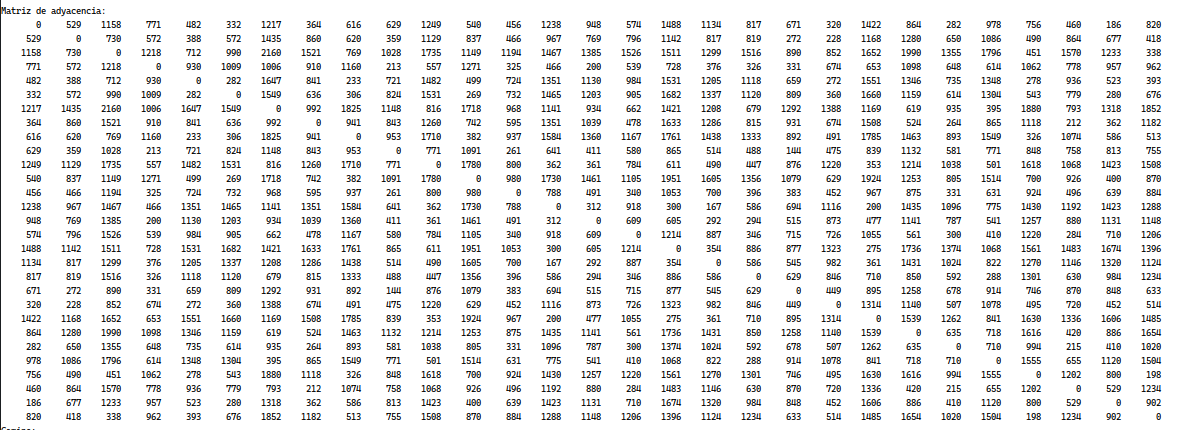
\includegraphics[scale=0.5]{img/ady-bayg.png}
  \caption{Matriz de adyacencia para el caso bayg.}
\end{figure}

\begin{figure}[H]
  \centering
  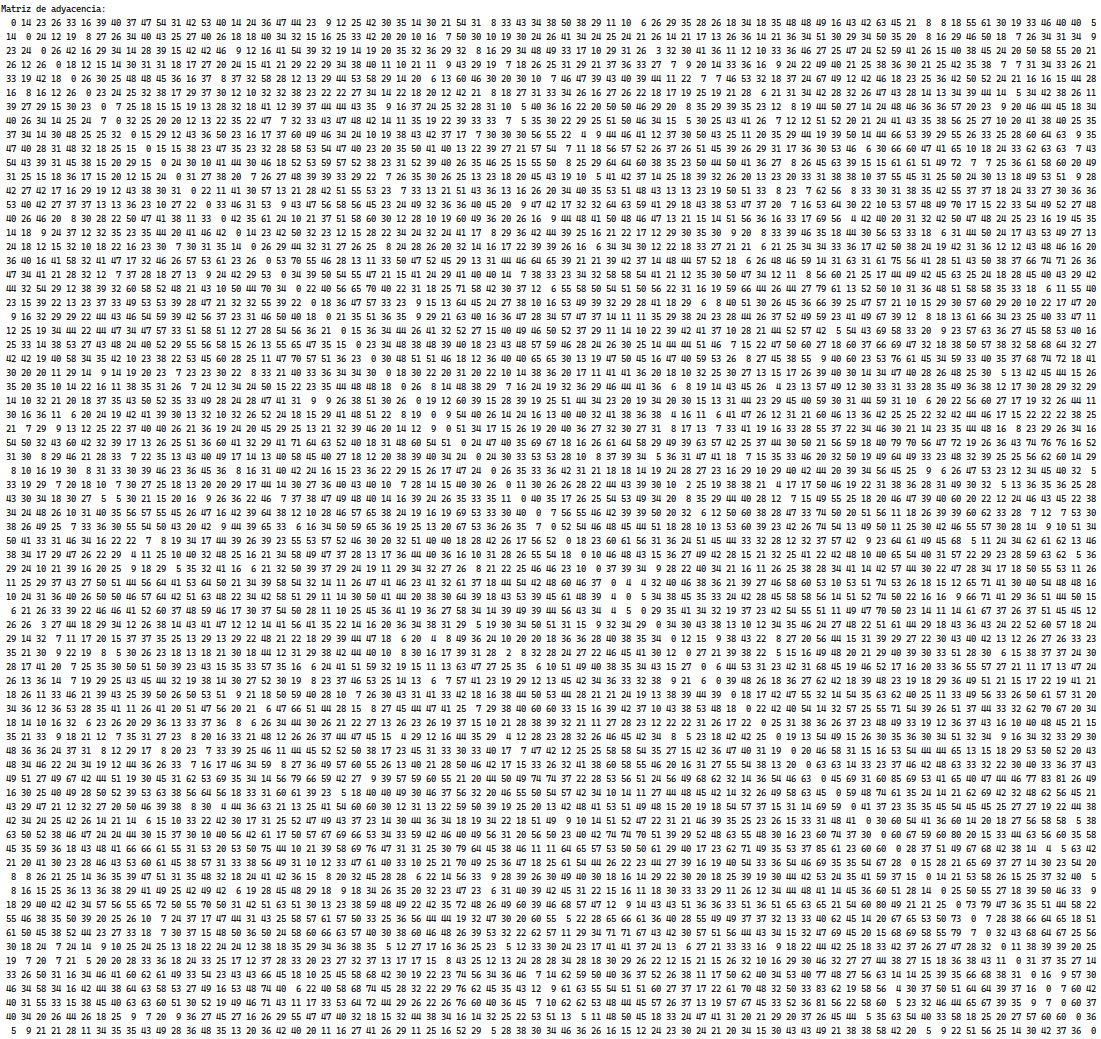
\includegraphics[scale=0.5]{img/ady-eil.png}
  \caption{Matriz de adyacencia para el caso eil.}
\end{figure}

\begin{figure}[H]
  \centering
  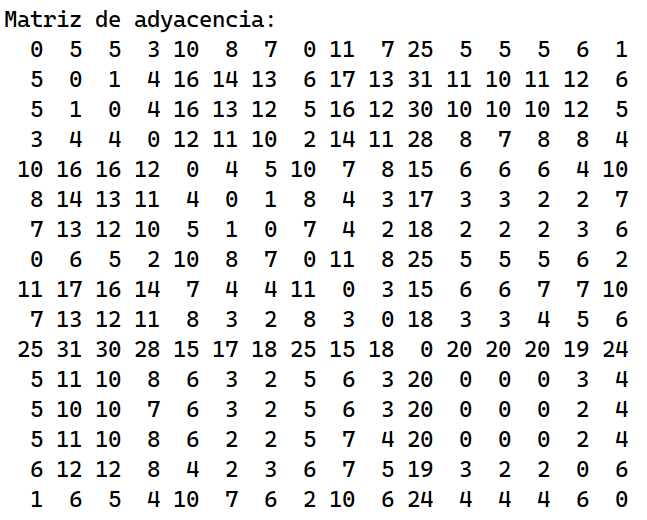
\includegraphics[scale=0.5]{img/ady-ulysses.png}
  \caption{Matriz de adyacencia para el caso ulysses.}
\end{figure}

En la siguiente tabla quedan recogidas las distancias calculadas por cada una de las heurísticas.

\begin{table}[H]
    \centering
    \begin{tabular}{|c|c|c|c|}
      \hline
      & bayg & eil & ulysses \\
      \hline
      vecino más cercano & 10200 & 662 & 79 \\
      \hline
      inserción & 9607 & 575 & 70 \\
      \hline
      $\alpha$-Kruskal & 10845 & 710 & 78 \\
      \hline
    \end{tabular}
    \caption{Tabla donde se indica la distancia total del ciclo recorrido en los conjuntos de prueba
    en función de la heurística empleada.}
\end{table}

\begin{figure}[H]
  \centering
  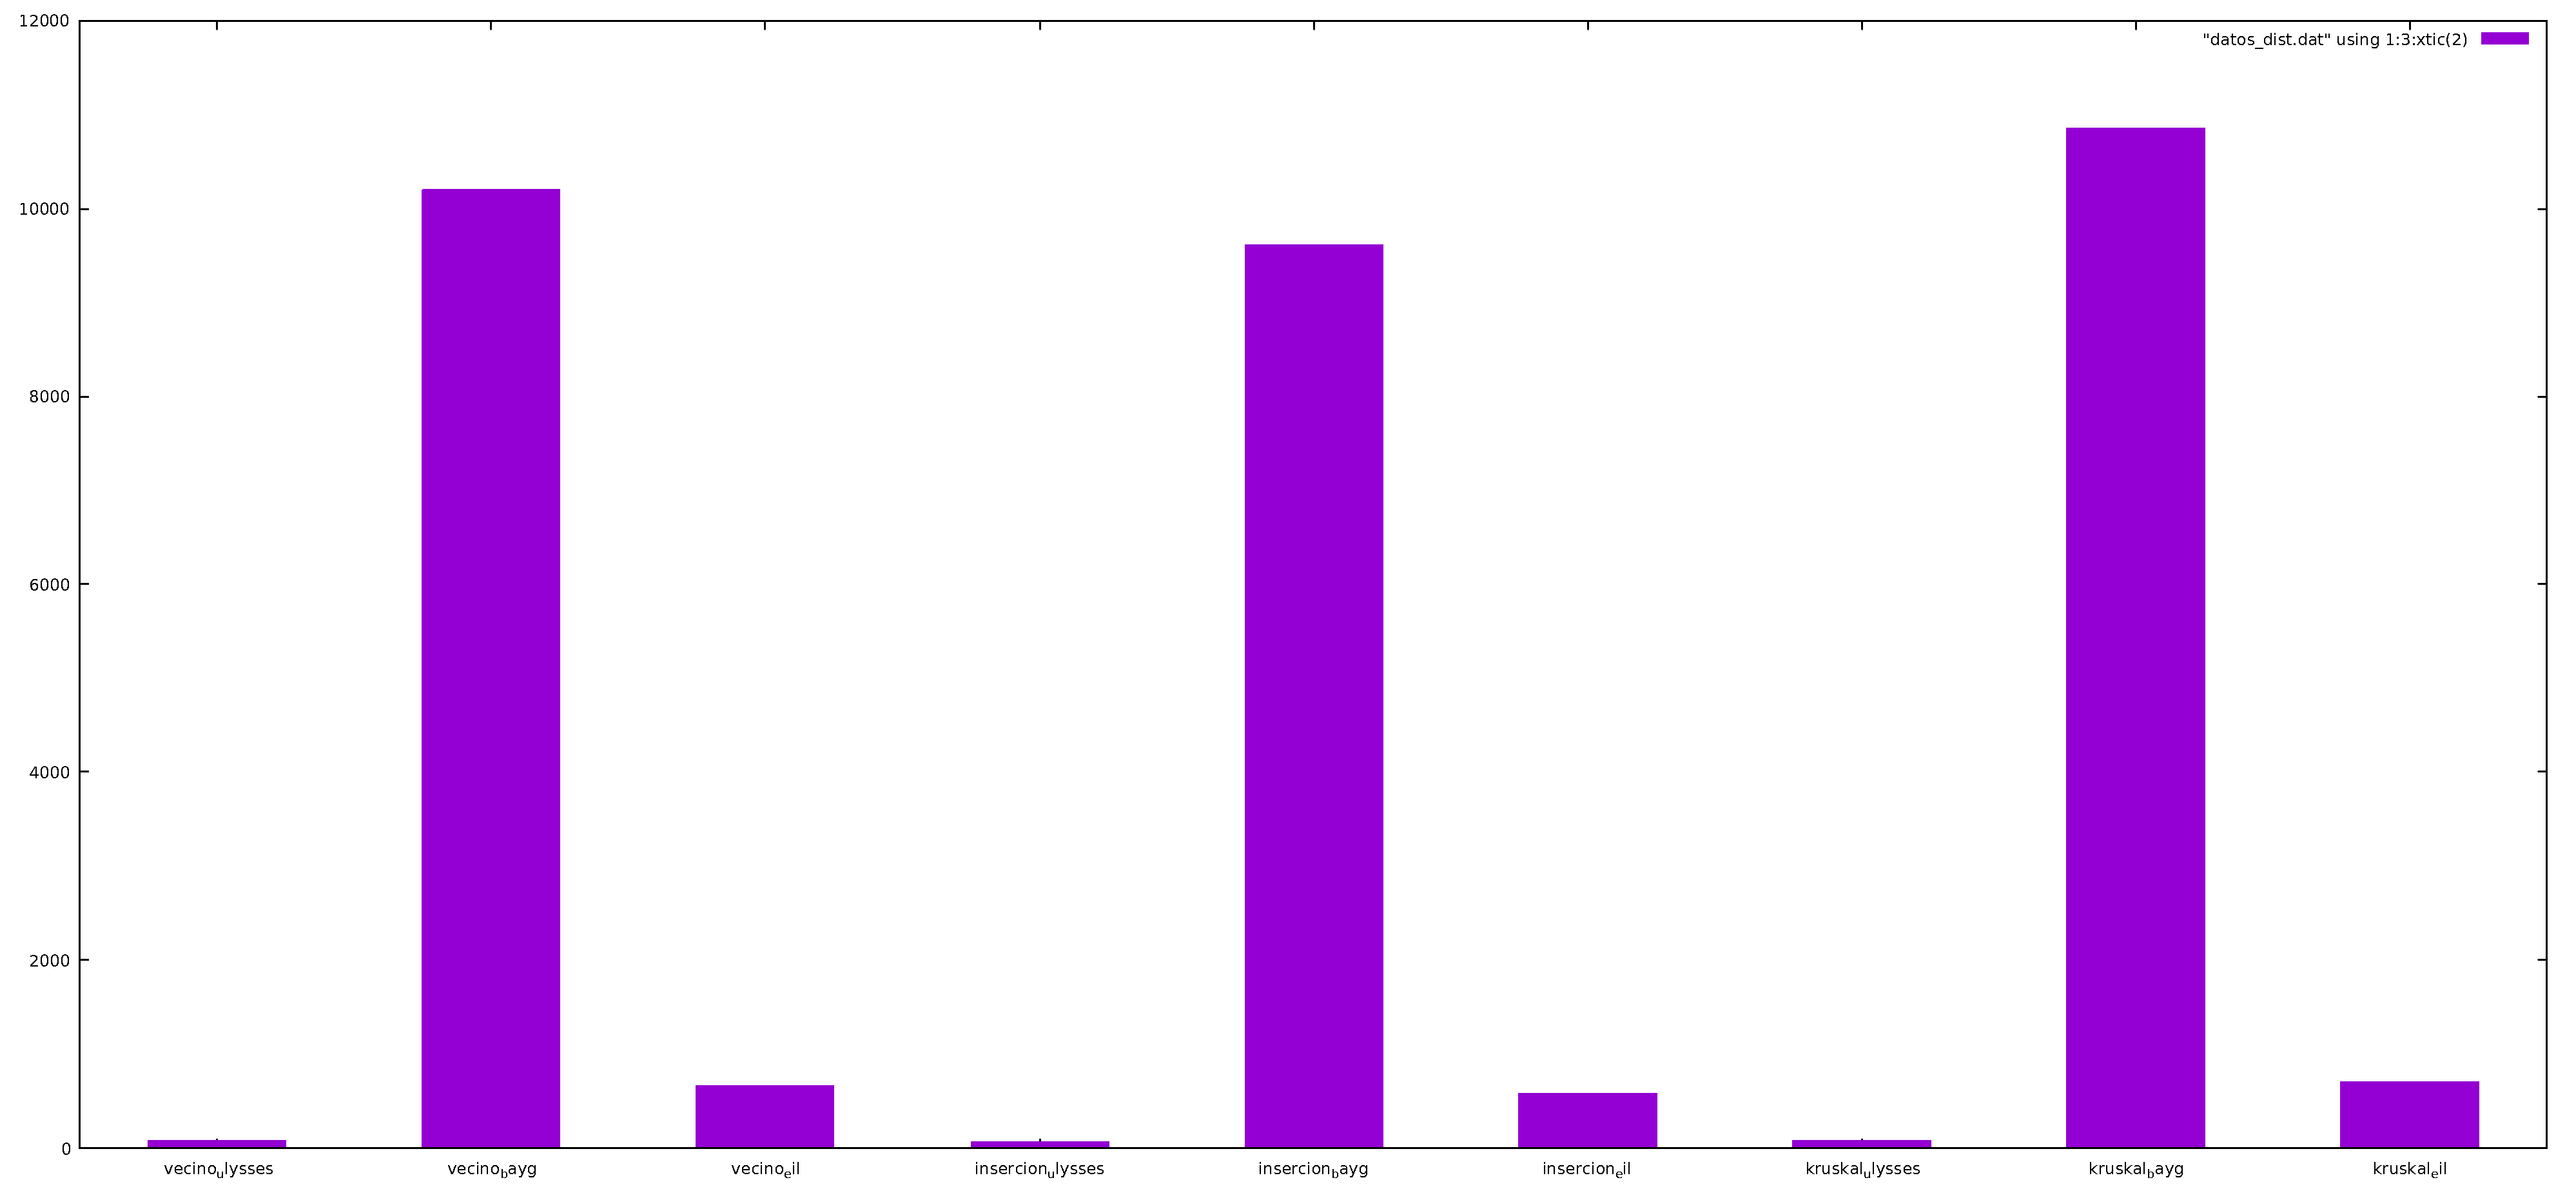
\includegraphics[scale=0.15]{../src/Comparacion_distancias.pdf}
  \caption{Gŕafica de barras donde se indica la distancia total del ciclo recorrido en los conjuntos de prueba en función de la heurística empleada.}
\end{figure}

También se han adjuntado capturas con cada una de las ejecuciones realizadas, mostrándose tanto la suma
total como el camino recorrido.

\begin{figure}[H]
  \centering
  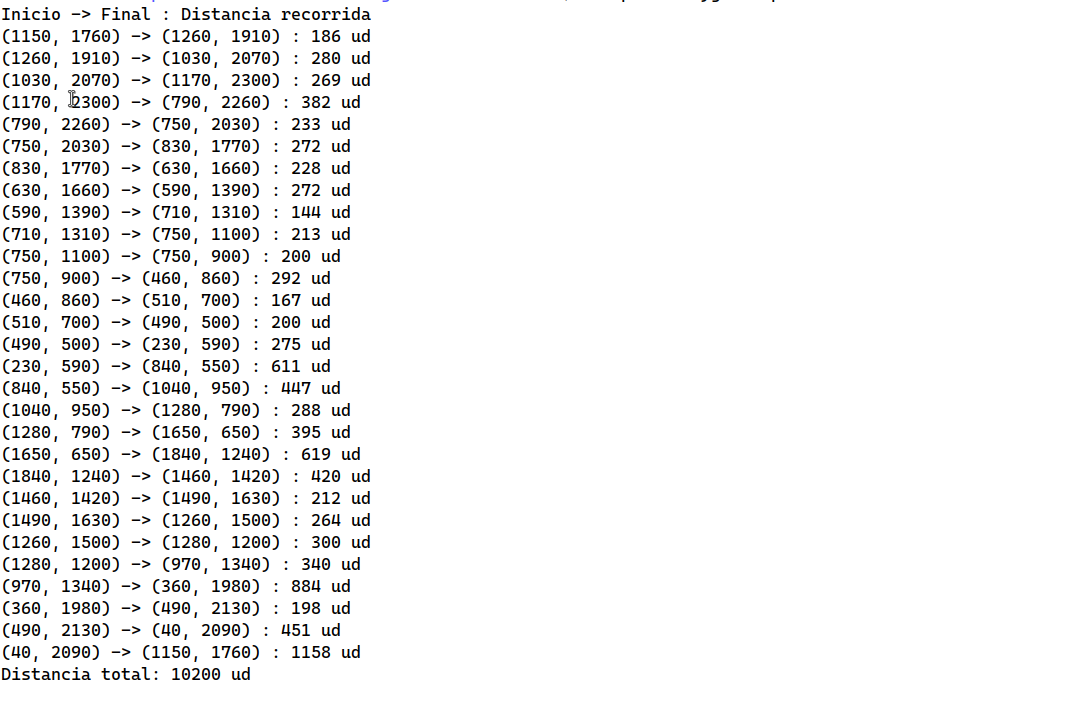
\includegraphics[scale=0.7]{img/dist-vecinos-bayg.png}
  \caption{Camino generado por la heurística del vecino más cercano en bayg.}
\end{figure}

\begin{figure}[H] 
  \centering
  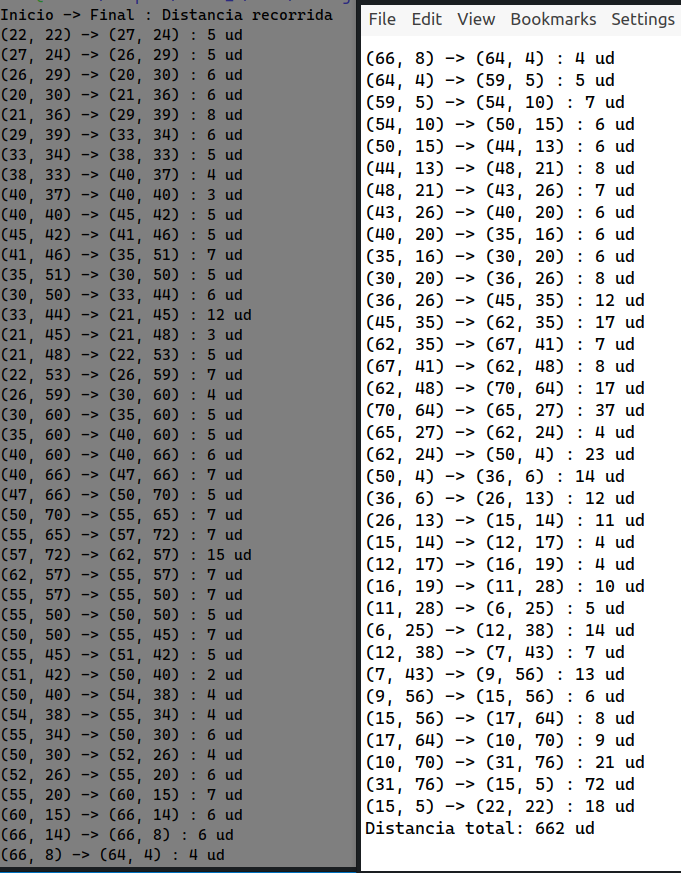
\includegraphics[scale=0.5]{img/dist-vecinos-eil.png}
  \caption{Camino generado por la heurística del vecino más cercano en eil.}
\end{figure}

\begin{figure}[H] 
  \centering
  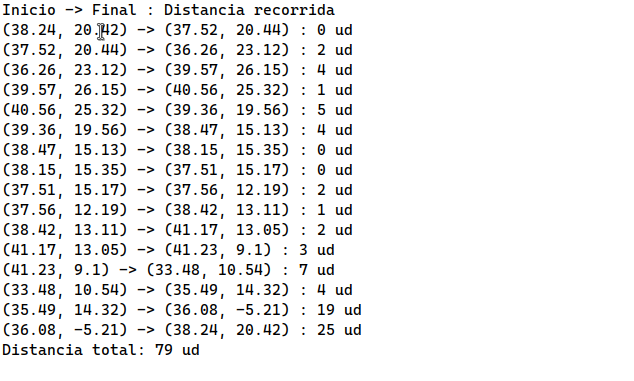
\includegraphics[scale=0.5]{img/dist-vecino-ulysses.png}
  \caption{Camino generado por la heurística del vecino más cercano en ulysses.}
\end{figure}

\begin{figure}[H]
  \centering
  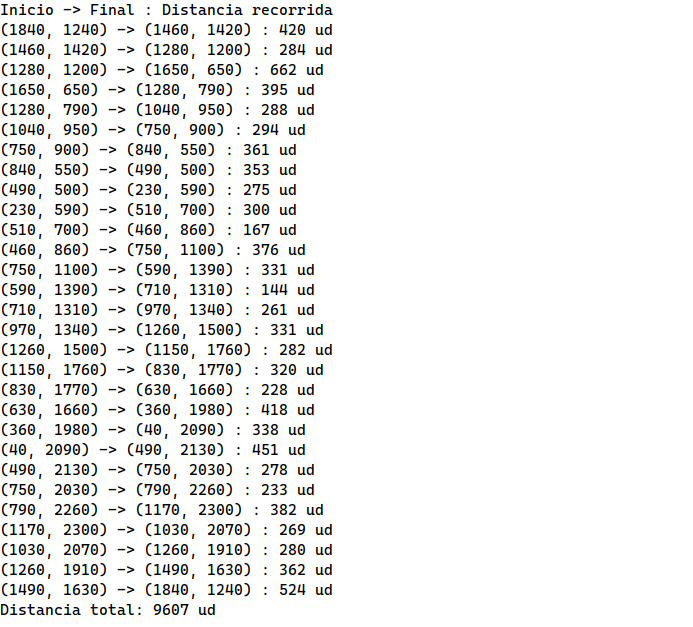
\includegraphics[scale=0.5]{img/dist-insercion-bayg.png}
  \caption{Camino generado por la heurística de la inserción más económica en bayg.}
\end{figure}

\begin{figure}[H]
  \centering
  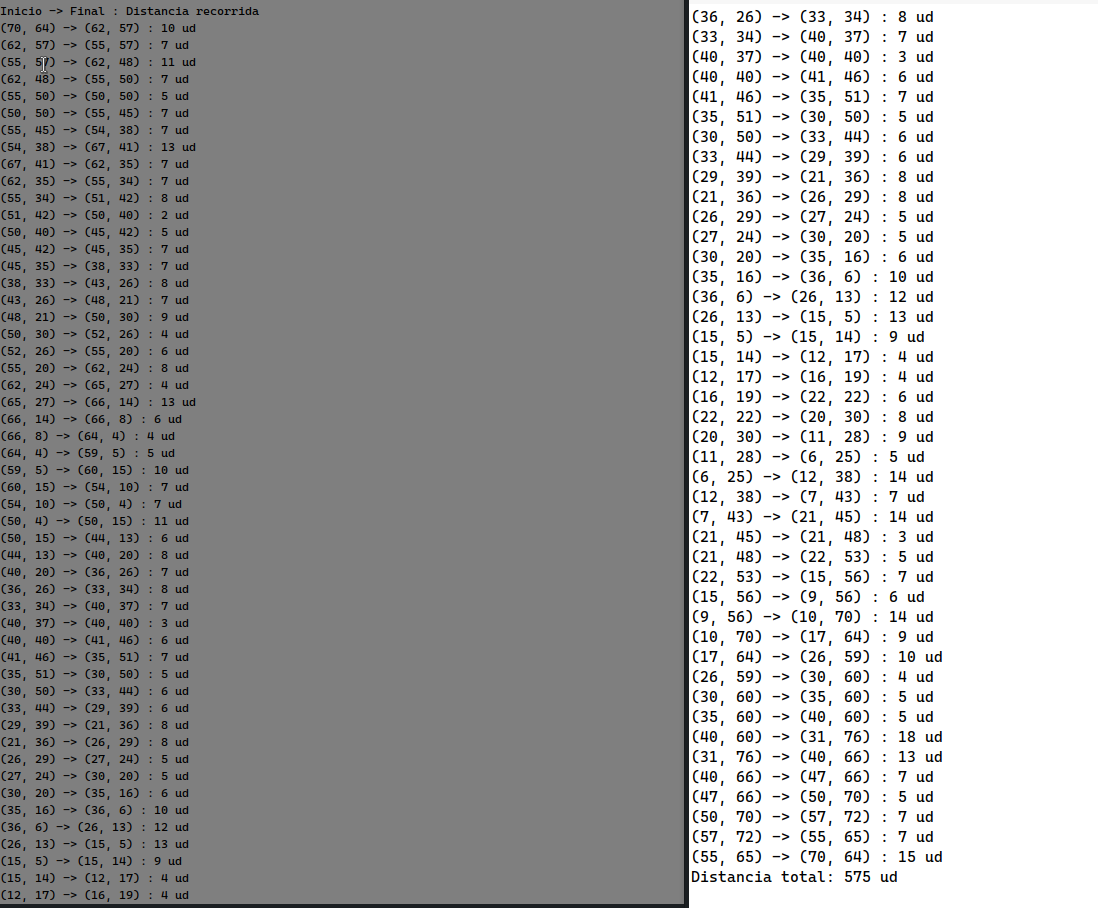
\includegraphics[scale=0.5]{img/dist-insercion-eil.png}
  \caption{Camino generado por la heurística de la inserción más económica en eil.}
\end{figure}

\begin{figure}[H]
  \centering
  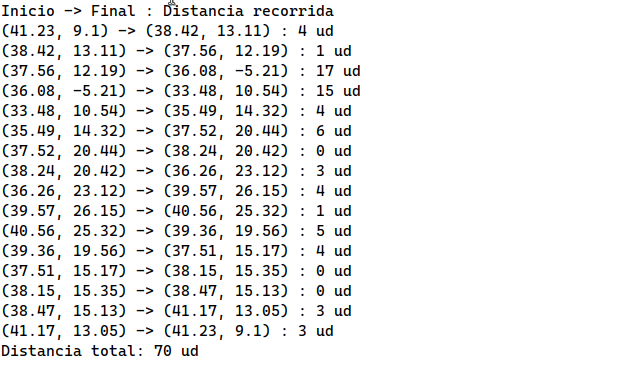
\includegraphics[scale=0.5]{img/dist-insercion-ulysses.png}
  \caption{Camino generado por la heurística de la inserción más económica en ulysses.}
\end{figure}

\begin{figure}[H]
  \centering
  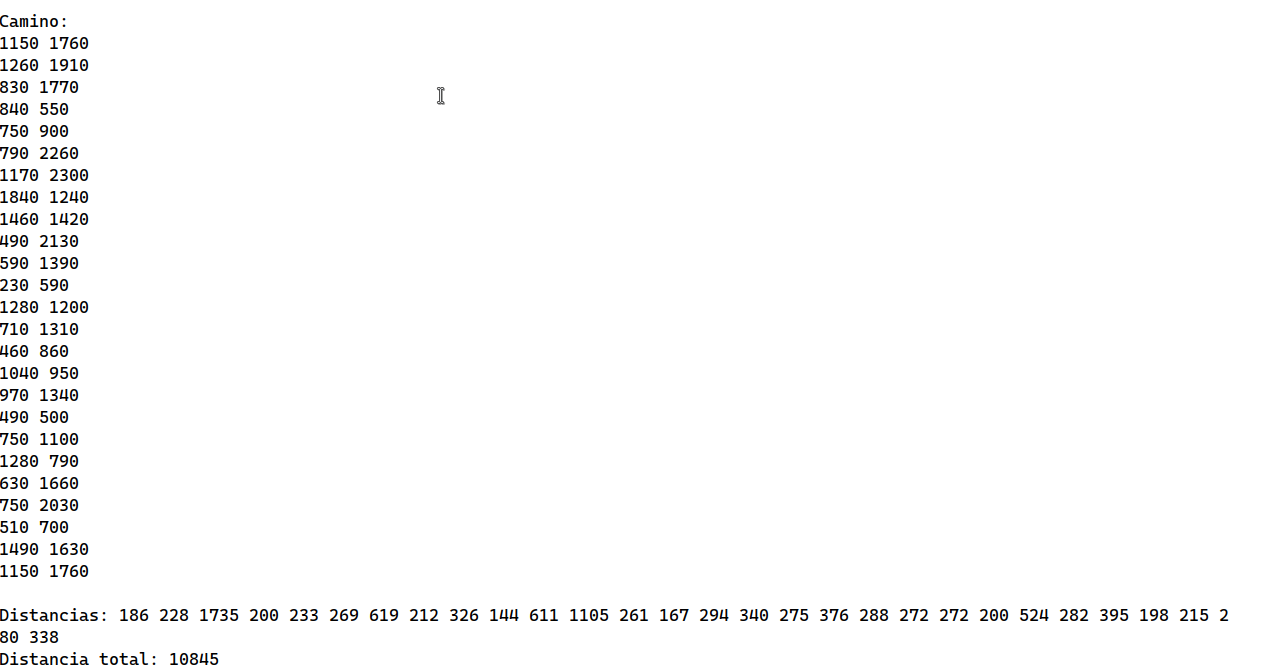
\includegraphics[scale=0.5]{img/dist-kr-bayg.png}
  \caption{Camino generado por la heurística propia en bayg.}
\end{figure}

\begin{figure}[H]
  \centering
  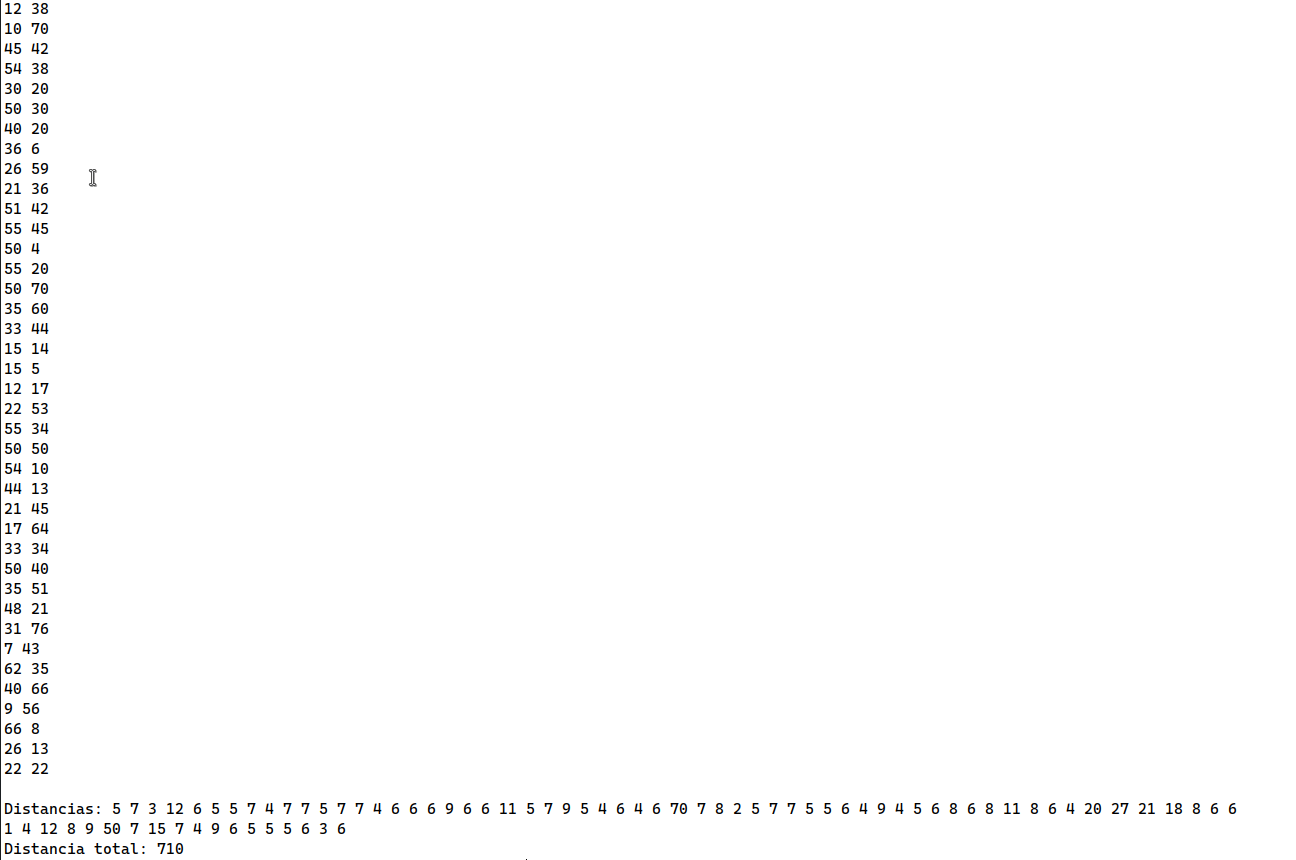
\includegraphics[scale=0.5]{img/dist-kr-eil.png}
  \caption{Camino generado por la heurística propia en eil.}
\end{figure}

\begin{figure}[H]
  \centering
  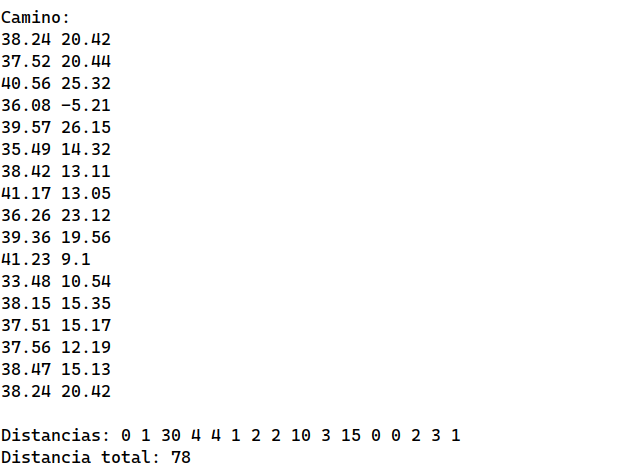
\includegraphics[scale=0.5]{img/dist-kr-ulysses.png}
  \caption{Camino generado por la heurística propia en ulysses.}
\end{figure} 

A continuación se adjuntan también las representaciones gráficas de cada
uno de los caminos de que realizan los algoritmos.

\begin{figure}[H]
  \centering
  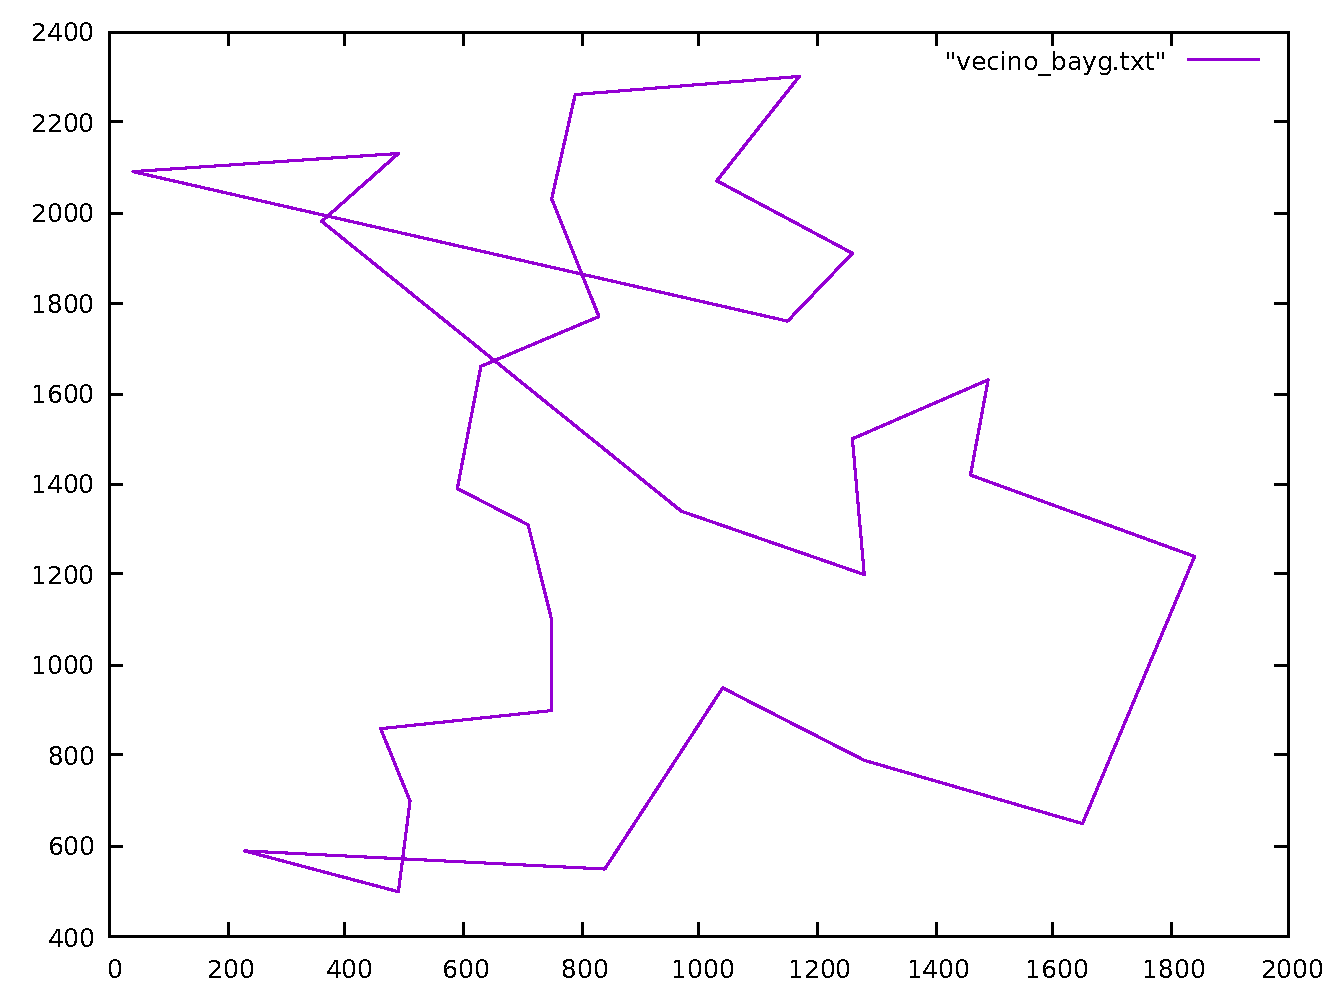
\includegraphics[scale=0.5]{../src/vecino_bayg.pdf}
  \caption{Representación gráfica del camino generado por la heurística del vecino más cercano en bayg.}
\end{figure} 

\begin{figure}[H]
  \centering
  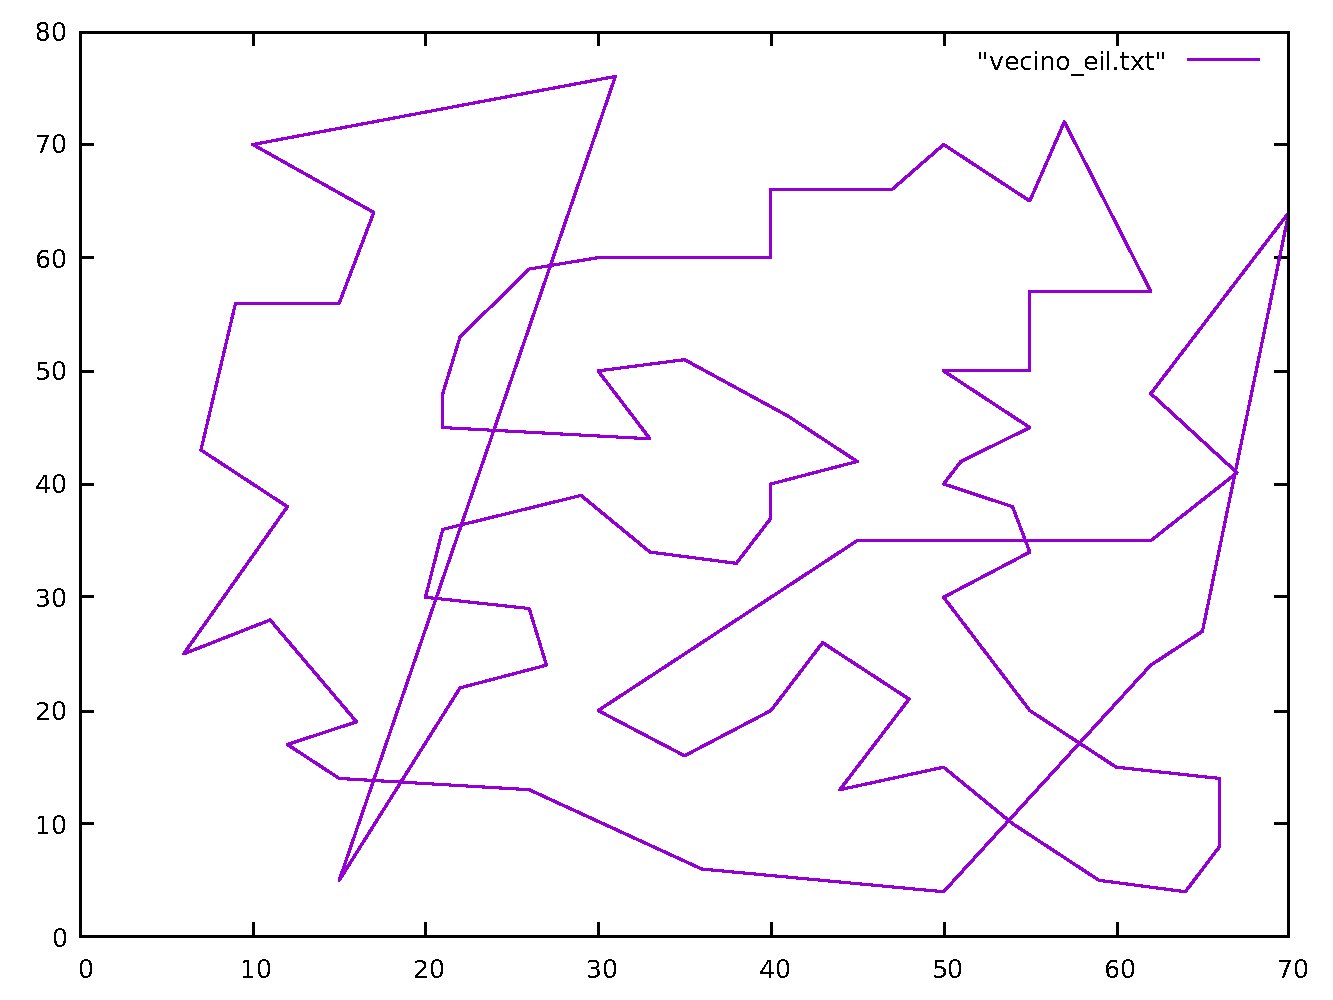
\includegraphics[scale=0.5]{../src/vecino_eil.pdf}
  \caption{Representación gráfica del camino generado por la heurística del vecino más cercano en eil.}
\end{figure} 

\begin{figure}[H]
  \centering
  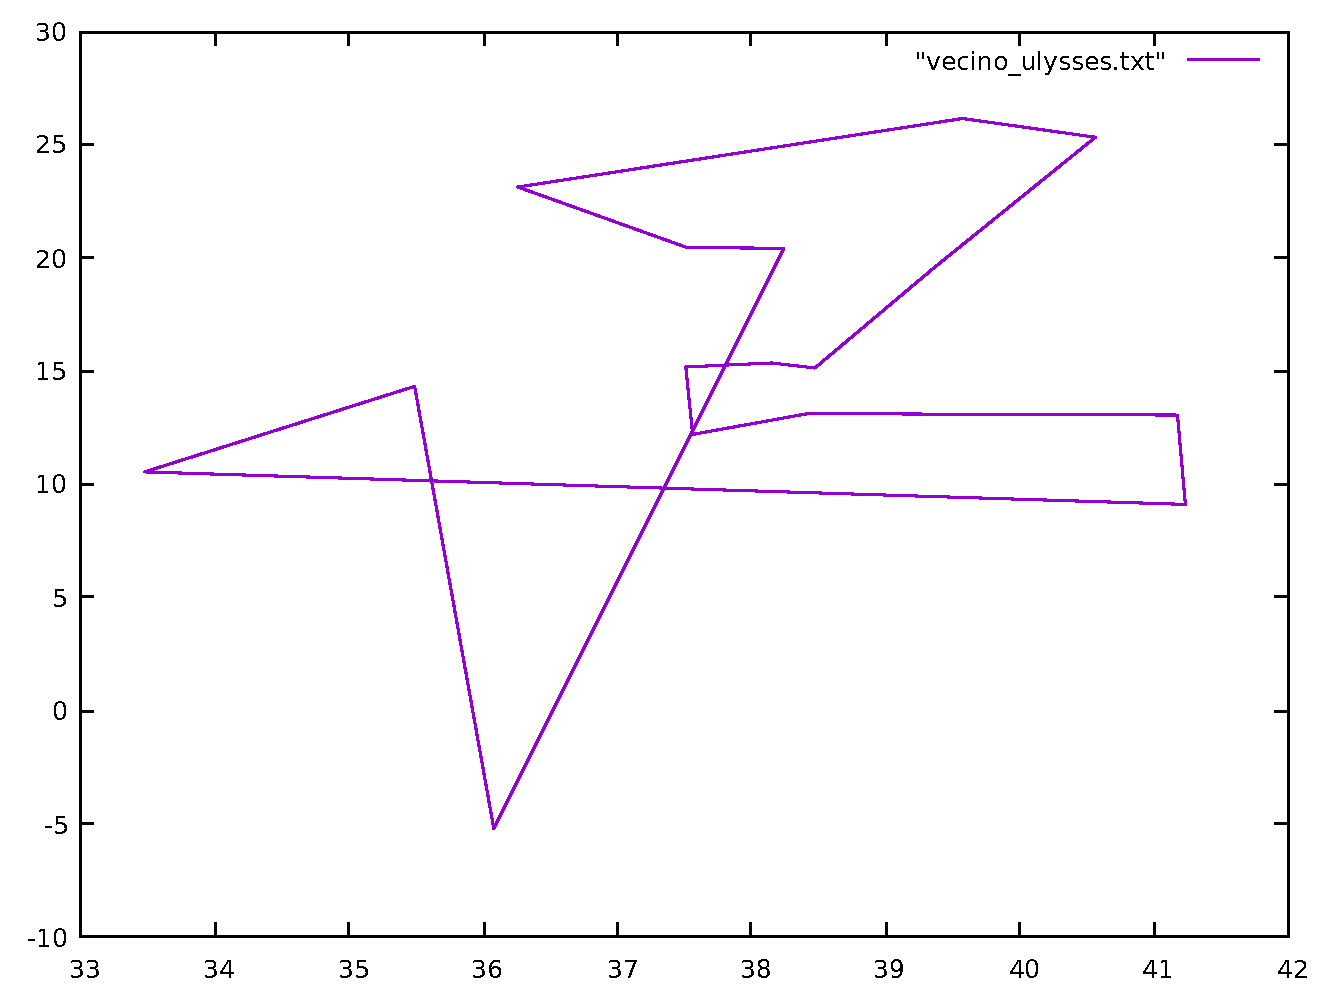
\includegraphics[scale=0.5]{../src/vecino_ulysses.pdf}
  \caption{Representación gráfica del camino generado por la heurística del vecino más cercano en ulysses.}
\end{figure} 

\begin{figure}[H]
  \centering
  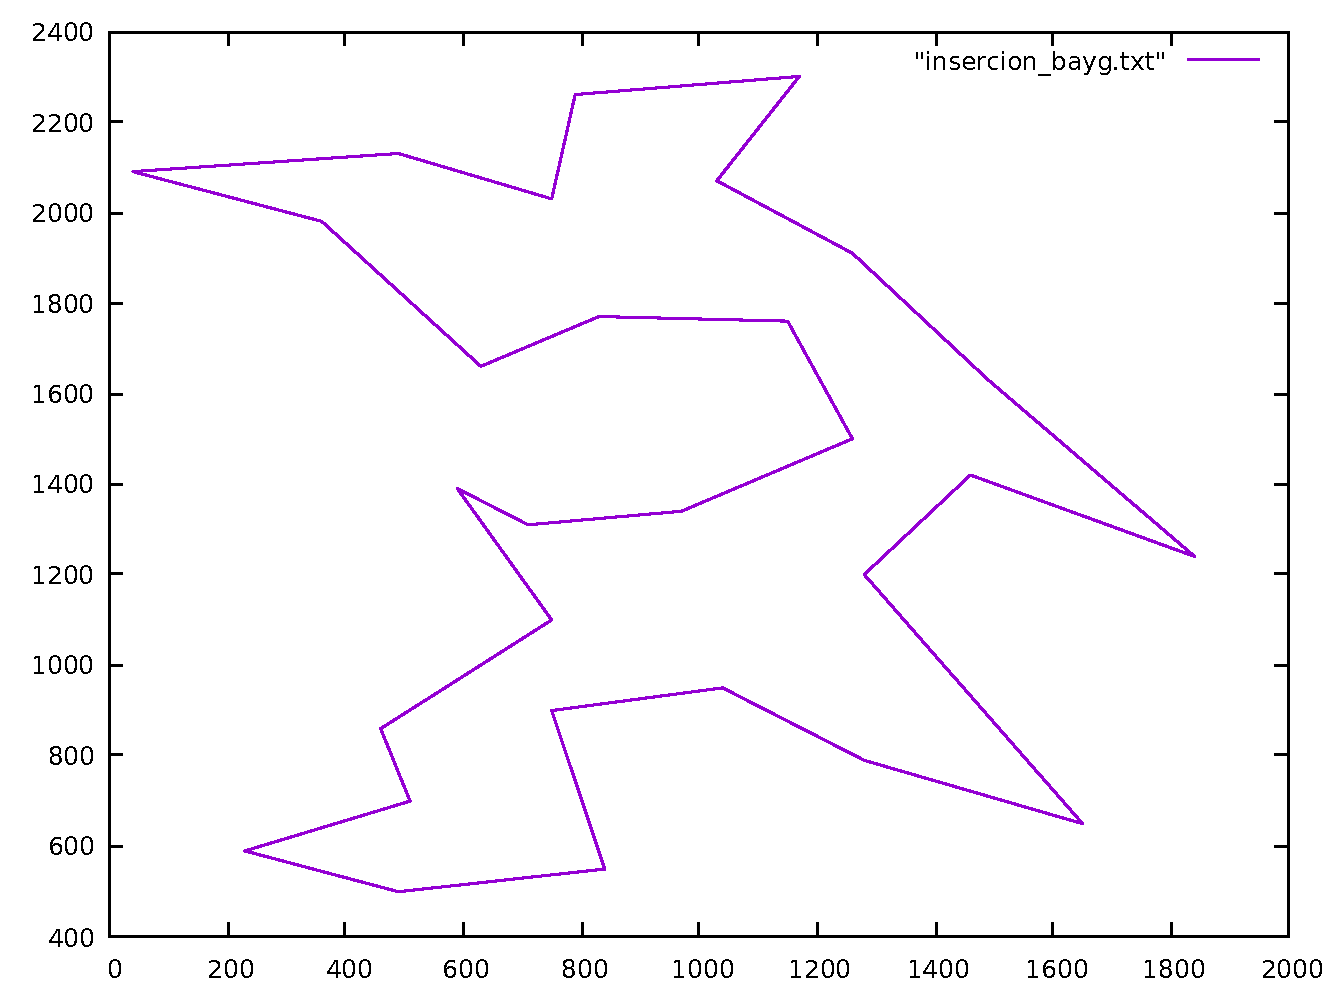
\includegraphics[scale=0.5]{../src/insercion_bayg.pdf}
  \caption{Representación gráfica del camino generado por la heurística de inserción económica en bayg.}
\end{figure} 

\begin{figure}[H]
  \centering
  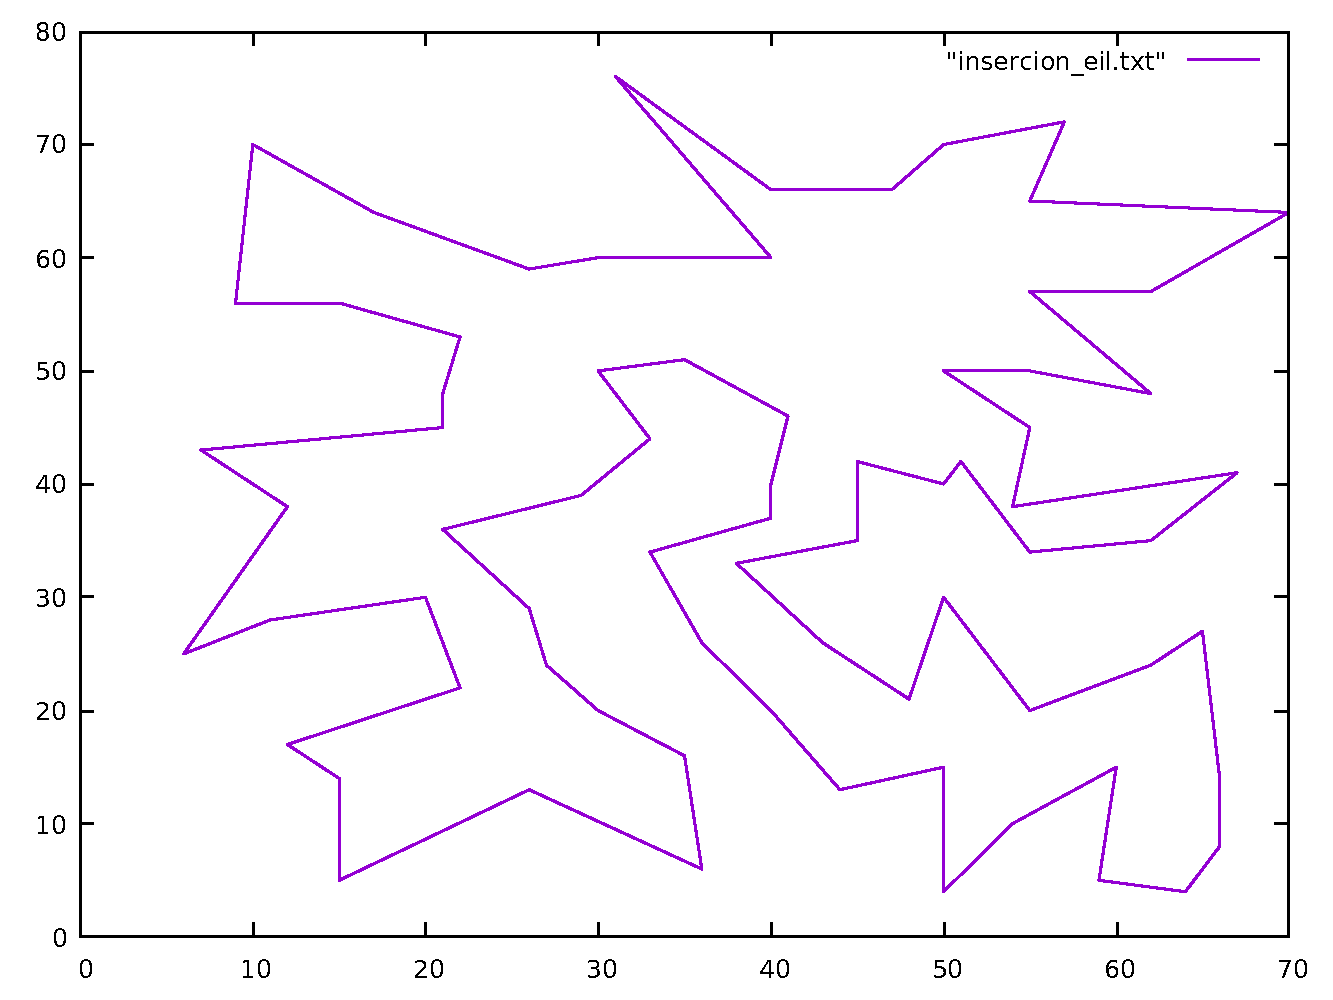
\includegraphics[scale=0.5]{../src/insercion_eil.pdf}
  \caption{Representación gráfica del camino generado por la heurística de inserción económica en eil.}
\end{figure}

\begin{figure}[H]
  \centering
  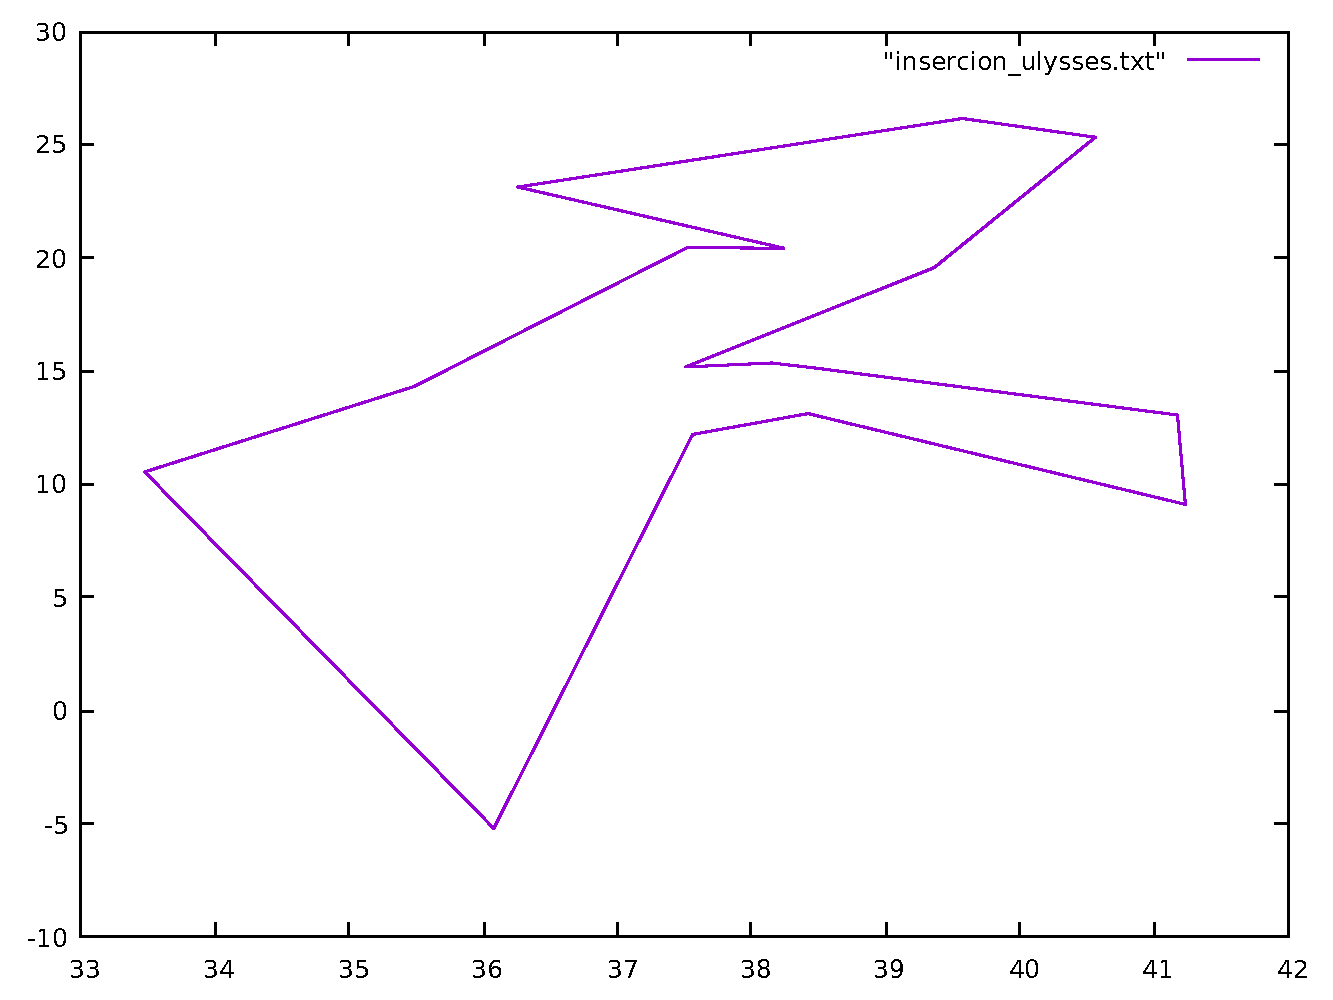
\includegraphics[scale=0.5]{../src/insercion_ulysses.pdf}
  \caption{Representación gráfica del camino generado por la heurística de inserción económica en ulysses.}
\end{figure} 

\begin{figure}[H]
  \centering
  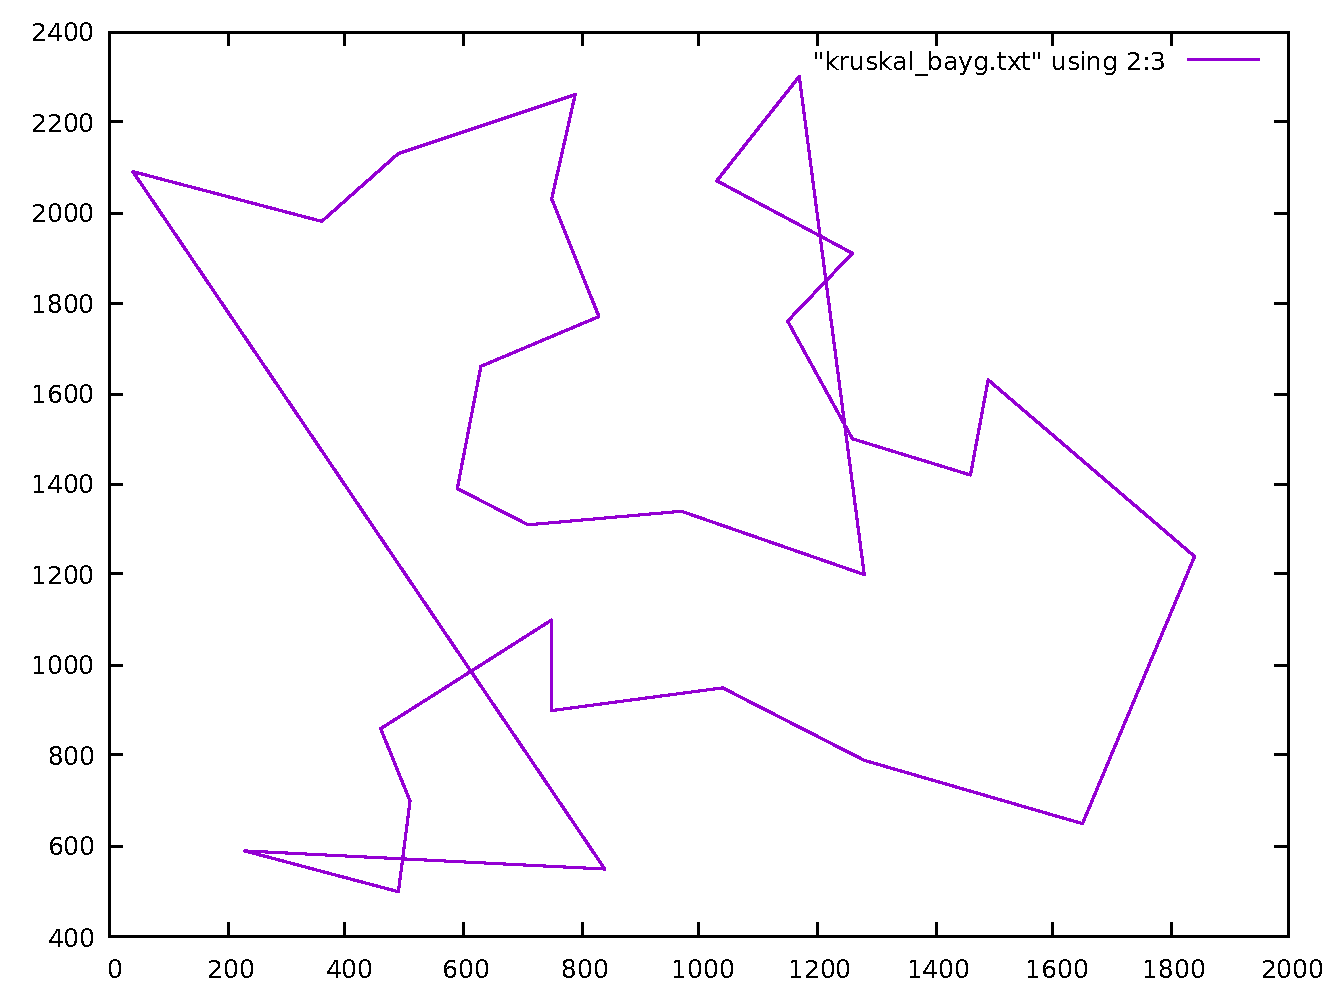
\includegraphics[scale=0.5]{../src/kruskal_bayg.pdf}
  \caption{Representación gráfica del camino generado por la heurística $\alpha$-Kruskal en bayg.}
\end{figure} 

\begin{figure}[H]
  \centering
  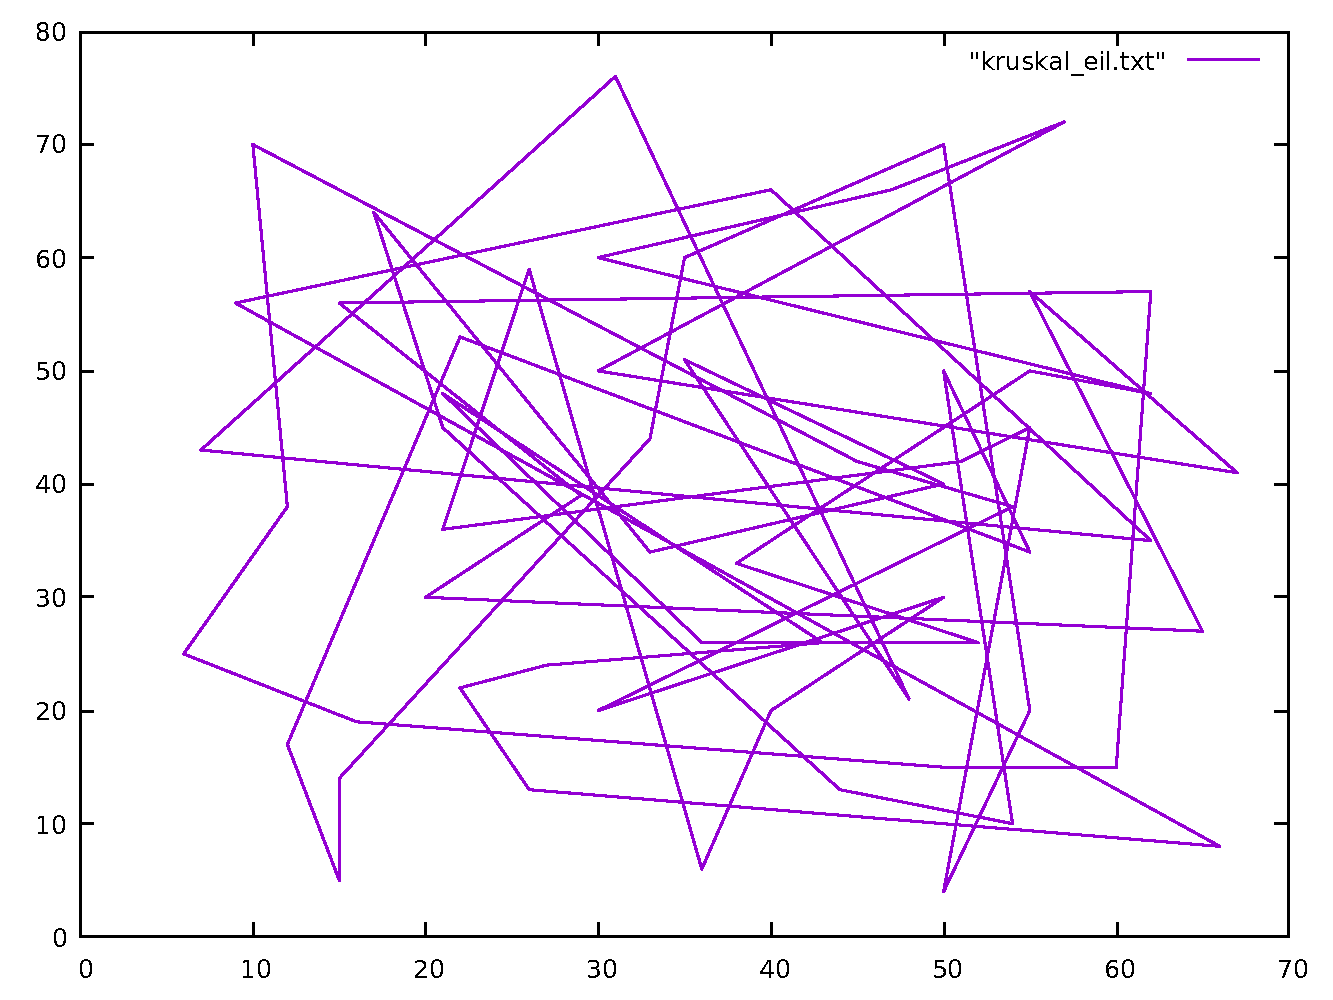
\includegraphics[scale=0.5]{../src/kruskal_eil.pdf}
  \caption{Representación gráfica del camino generado por la heurística $\alpha$-Kruskal en eil.}
\end{figure} 

\begin{figure}[H]
  \centering
  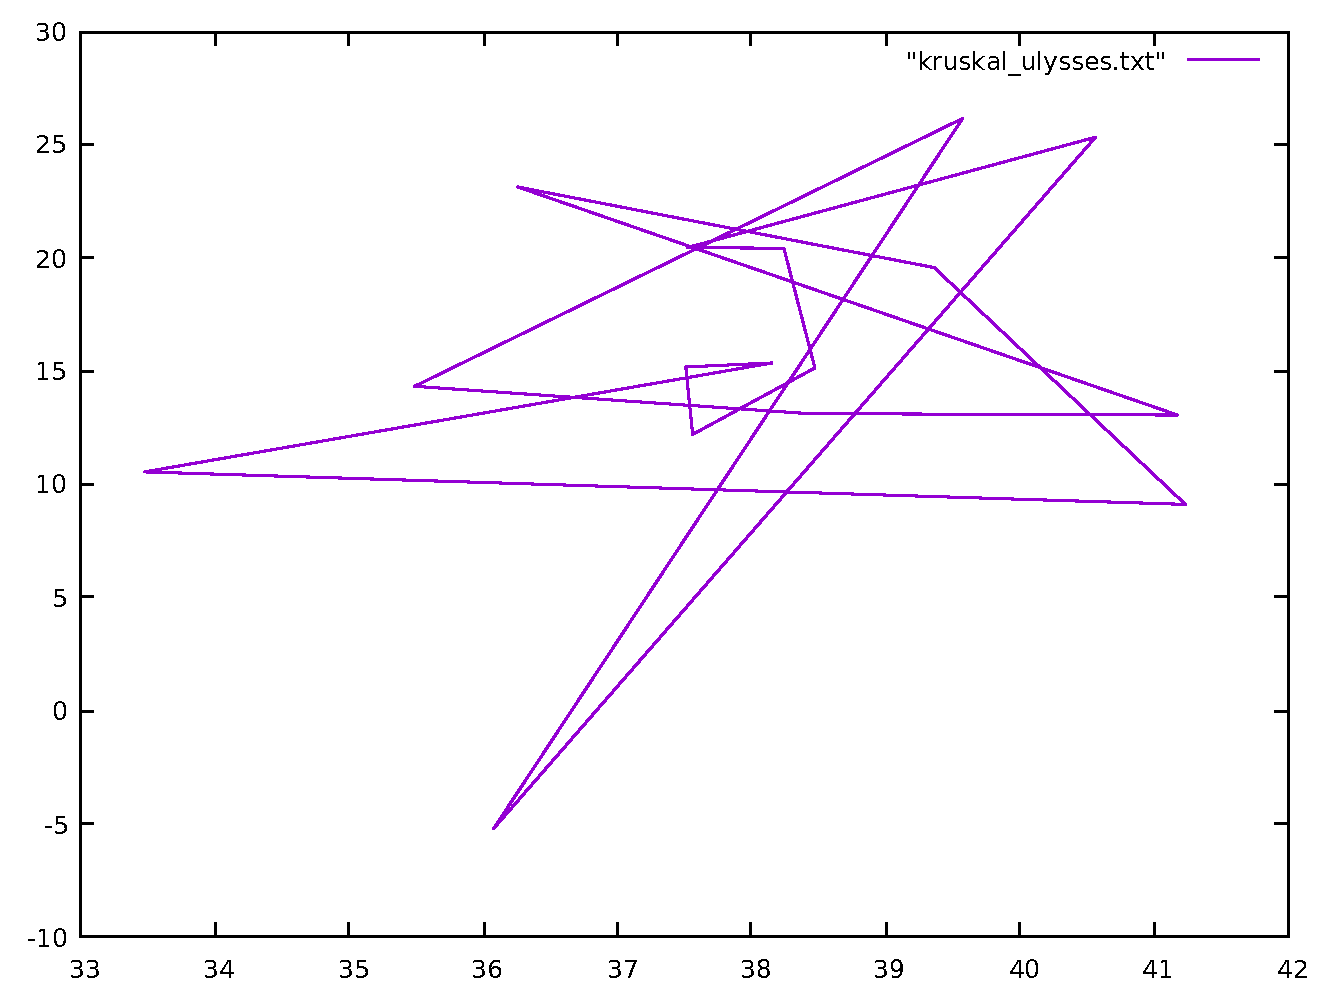
\includegraphics[scale=0.5]{../src/kruskal_ulysses.pdf}
  \caption{Representación gráfica del camino generado por la heurística $\alpha$-Kruskal en ulysses.}
\end{figure} 